\documentclass[11pt]{article}
\usepackage[utf8]{inputenc}
\usepackage[T1]{fontenc}
\usepackage{amsmath}
\usepackage{amssymb}
\usepackage{multicol}
\usepackage{geometry}
\usepackage{tikz}
\usepackage{enumitem}
\usepackage{xcolor}
\usepackage{titlesec}
\usepackage{graphicx} % no preâmbulo

% Configurações de layout
\geometry{a4paper, left=1cm, right=1cm, top=0.5cm, bottom=1.2cm}
\setlength{\columnseprule}{0.4pt}

% Cores para títulos
\titleformat{\section}{\normalfont\Large\bfseries\color{blue}}{\thesection}{1em}{}
\titleformat{\subsection}{\normalfont\large\bfseries\color{red}}{\thesubsection}{1em}{}

\title{\textcolor{blue}{Terceiro Trimestre: Matemática Básica \\
Medidas de Tendência Central e Porcentagem}}
\author{Professor: Jefferson}
\date{}

\begin{document}

\maketitle
\vspace{-1cm}

\begin{center}
\large{Nome: \underline{\hspace{8cm}} \quad Turma: \underline{\hspace{3cm}}}
\end{center}

\begin{multicols}{2}

\section*{Objetivo da Aula}

% CAIXA COLORIDA COM A HABILIDADE
\begin{tikzpicture}
\node[rectangle, 
      fill=purple!15, 
      rounded corners=5pt, 
      inner sep=10pt, 
      draw=purple!60!black, 
      thick,
      drop shadow={opacity=0.3}] (box) 
{
\begin{minipage}{0.75\linewidth}
\justifying
\small
\textbf{(EM13MAT316PE32)} Resolver e elaborar situações problema, em contextos diversos, que envolvam o cálculo e a interpretação das medidas de tendência central (média, moda, mediana) e das medidas de dispersão (amplitude, variância e desvio padrão), com e/ou sem apoio de tecnologias digitais.
\end{minipage}
};
\end{tikzpicture}

\vspace{5mm}

\section*{1. Medidas de Tendência Central}

\subsection*{Média Aritmética ($\bar{x}$)}

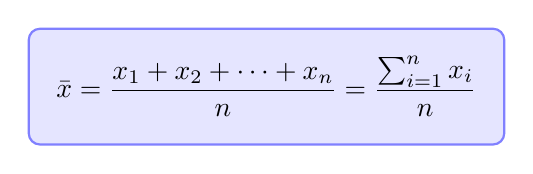
\begin{tikzpicture}
\node[rectangle, fill=blue!10, rounded corners, inner sep=10pt, draw=blue!50, thick] (box) {
$\displaystyle \bar{x} = \frac{x_1 + x_2 + \cdots + x_n}{n} = \frac{\sum_{i=1}^{n} x_i}{n}$
};
\end{tikzpicture}

\vspace{5mm}

\textbf{Onde:}
\begin{itemize}
\item $\textcolor{red}{x_i}$ = cada valor do conjunto
\item $\textcolor{red}{n}$ = número total de valores
\end{itemize}

\subsection*{Exemplo:}
Calcule a média das notas: 7, 8, 6, 9, 5
\[
\bar{x} = \frac{7 + 8 + 6 + 9 + 5}{5} = \frac{35}{5} = 7
\]

\subsection*{Moda (Mo)}

\resizebox{1.0\linewidth}{!}{%
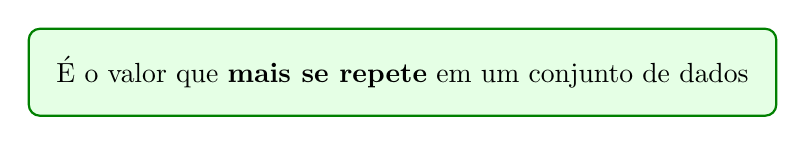
\begin{tikzpicture}
\node[rectangle, fill=green!10, rounded corners, inner sep=10pt, draw=green!50!black, thick] (box) {
É o valor que \textbf{mais se repete} em um conjunto de dados
};
\end{tikzpicture}
    }

\vspace{5mm}

\textbf{Tipos:}
\begin{itemize}
\item \textbf{Amodal}: nenhum valor se repete
\item \textbf{Unimodal}: apenas uma moda
\item \textbf{Bimodal}: duas modas
\item \textbf{Multimodal}: três ou mais modas
\end{itemize}

\subsection*{Exemplo:}
\begin{itemize}
\item Conjunto A: 2, 3, 5, 7, 8 → \textbf{Amodal}
\item Conjunto B: 4, 5, 5, 6, 7 → \textbf{Moda = 5}
\item Conjunto C: 2, 3, 3, 4, 4, 5 → \textbf{Bimodal: 3 e 4}
\end{itemize}

\subsection*{Mediana (Md)}

\resizebox{1.1\linewidth}{!}{%
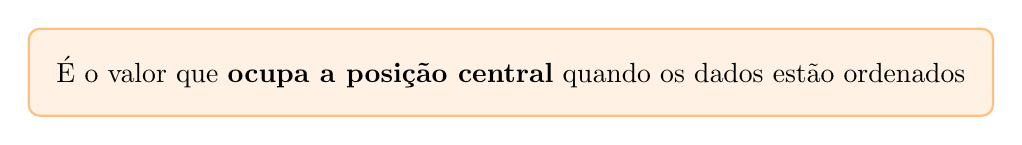
\begin{tikzpicture}
\node[rectangle, fill=orange!10, rounded corners, inner sep=10pt, draw=orange!50, thick] (box) {
É o valor que \textbf{ocupa a posição central} quando os dados estão ordenados
};
\end{tikzpicture}%
}

\vspace{5mm}

\textbf{Como calcular:}
\begin{enumerate}
\item Ordene os dados em ordem crescente
\item Se $n$ é ímpar: $Md =$ valor central
\item Se $n$ é par: $Md =$ média dos dois valores centrais
\end{enumerate}

\subsection*{Exemplo:}
\begin{itemize}
\item Conjunto ímpar: 3, 5, 7, 9, 11 → $Md = 7$
\item Conjunto par: 2, 4, 6, 8, 10, 12 → $Md = \frac{6 + 8}{2} = 7$
\end{itemize}

\section*{2. Porcentagem}

\subsection*{O que é porcentagem?}

\resizebox{1.1\linewidth}{!}{%
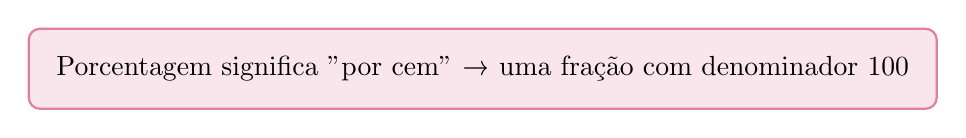
\begin{tikzpicture}
\node[rectangle, fill=purple!10, rounded corners, inner sep=10pt, draw=purple!50, thick] (box) {
Porcentagem significa "por cem" → uma fração com denominador 100
};
\end{tikzpicture}
}

\vspace{5mm}

\[
p\% = \frac{p}{100}
\]

\subsection*{Cálculos Básicos}

\begin{align*}
\text{Calcular } p\% \text{ de um valor} &: valor \times \frac{p}{100} \\
\text{Calcular qual } \% \text{ um valor representa} &: \frac{valor}{total} \times 100\% \\
\text{Aumento de } p\% &: valor \times (1 + \frac{p}{100}) \\
\text{Desconto de } p\% &: valor \times (1 - \frac{p}{100})
\end{align*}

\subsection*{Exemplo Prático:}
Um produto custa R\$ 80,00. Com 15\% de desconto:
\[
Novo\ preço = 80 \times (1 - \frac{15}{100}) = 80 \times 0,85 = R\$ 68,00
\]

\section*{3. Aplicações Práticas}

\subsection*{Exemplo 1: Análise de Notas}

As notas de uma turma foram: 5, 6, 6, 7, 7, 7, 8, 8, 9, 10

\textbf{Cálculos:}
\begin{itemize}
\item \textbf{Média}: $\frac{5+6+6+7+7+7+8+8+9+10}{10} = \frac{73}{10} = 7,3$
\item \textbf{Moda}: 7 (aparece 3 vezes)
\item \textbf{Mediana}: $\frac{7+7}{2} = 7$ (valores centrais: 7 e 7)
\end{itemize}

\subsection*{Exemplo 2: Problema de Porcentagem}

Uma loja aumentou seus preços em 20\% e depois anunciou um desconto de 20\%. O preço voltou ao original?

\textbf{Solução:}
\begin{align*}
Preço\ original &= 100 \\
Após\ aumento &= 100 \times 1,20 = 120 \\
Após\ desconto &= 120 \times 0,80 = 96 \\
Resultado &= 96\%\ do\ original
\end{align*}
\textbf{Não voltou ao original!}

\section*{Exercícios}

\begin{enumerate}[leftmargin=*]

\item Calcule a média, moda e mediana dos conjuntos:
\begin{enumerate}[label=\alph*)]
\item 12, 15, 18, 12, 20, 15, 12
\item 7, 9, 11, 13, 15, 17
\item 5, 5, 8, 8, 8, 10, 10
\end{enumerate}

\item Um produto custava R\$ 250,00 e sofreu:
\begin{enumerate}[label=\alph*)]
\item Um aumento de 15\%
\item Dois aumentos consecutivos de 10\% cada
\item Um aumento de 20\% seguido de desconto de 15\%
\end{enumerate}
Calcule o preço final em cada caso.

\item Em uma turma de 40 alunos, 55\% são meninas. Quantos meninos há na turma?

\item As idades dos professores de uma escola são: 28, 32, 35, 35, 38, 40, 42, 45, 48, 52. Calcule:
\begin{enumerate}[label=\alph*)]
\item A idade média
\item A moda
\item A mediana
\end{enumerate}

\item Um investimento rendeu 8\% no primeiro mês, 12\% no segundo e 5\% no terceiro. Qual foi o rendimento total no trimestre?

\item (ENEM) Em uma pesquisa sobre preferência musical, 30\% dos entrevistados gostam de rock, 40\% de pop, 20\% de ambos os estilos. Qual a porcentagem que não gosta de nenhum desses estilos?

\item As alturas (em cm) de um time de basquete são: 185, 190, 192, 195, 198, 200, 205, 210. Calcule:
\begin{enumerate}[label=\alph*)]
\item A altura média
\item A mediana
\item A moda (se existir)
\end{enumerate}

\item Um comerciante comprou um produto por R\$ 80,00 e quer vendê-lo com lucro de 25\% sobre o preço de venda. Por quanto deve vender?

\item As notas de matemática de uma turma foram: 4, 5, 6, 6, 7, 7, 7, 8, 8, 9, 10. Se a média para aprovação é 7,0, quantos alunos foram aprovados?

\item (UERJ) Em uma liquidação, uma camisa que custava R\$ 120,00 foi vendida com 30\% de desconto. Se o comprador pagou com uma nota de R\$ 100,00, quanto recebeu de troco?

\end{enumerate}

\section*{4. Resolução de Problemas}

\subsection*{Problema 1: Análise Salarial}
Os salários de uma empresa são: R\$ 1200, R\$ 1500, R\$ 1800, R\$ 2000, R\$ 2000, R\$ 2200, R\$ 2500, R\$ 3000, R\$ 5000

\textbf{Calcule:}
\begin{enumerate}[label=\alph*)]
\item Média salarial
\item Mediana
\item Moda
\item Qual medida melhor representa o salário típico? Por quê?
\end{enumerate}

\subsection*{Problema 2: Descontos Sucessivos}
Uma loja anunciou: "30\% + 20\% de desconto = 50\% de desconto". Isso está correto?

\textbf{Resolução:}
\begin{align*}
Preço\ original &= 100 \\
1º\ desconto &= 100 \times 0,70 = 70 \\
2º\ desconto &= 70 \times 0,80 = 56 \\
Desconto\ total &= 100 - 56 = 44\% \\
\end{align*}
\textbf{Não equivale a 50\%!}

\end{multicols}

\end{document}
